\documentclass[tikz,border=5pt]{standalone}
\usepackage[UTF8]{ctex}
\usepackage{amsmath}
\usetikzlibrary{arrows.meta,calc}
\definecolor{blue}{RGB}{45,98,142}
\definecolor{red}{RGB}{175,67,51}
\definecolor{green}{RGB}{60,117,87}
\begin{document}
\begin{tikzpicture}
\draw[blue!30] (0,0)circle(3.2);
\draw[thick] (90:2.8)--(210:2.8)--(330:2.8)--cycle;
\foreach \ang in{30,150,270}{\draw[gray,dashed](0,0)--(\ang:1.4);\fill[blue](\ang:1.4)circle(3pt);\node at(\ang:1.75){$q$};}
\fill[red](0,0)circle(3pt);\node[below left]at(0,0){$-Q$};
\node[right]at(2.7,2){$\odot\ B=bt$};
\draw[blue,-{Stealth}](150:1.4)--++(.45,.78)node[left]{$x$};
\draw[gray,<->](-3,-1.3)--node[left]{$l$}(-.57,2.9);
\node at(0,-3.7){俯视图；绳沿三条槽边闭合};
\end{tikzpicture}
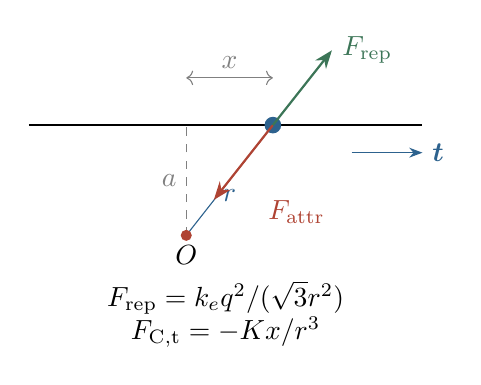
\begin{tikzpicture}
\coordinate(O)at(0,0);\coordinate(M)at(0,1.4);\coordinate(P)at(1.1,1.4);
\draw[thick](-2,1.4)--(3,1.4);
\draw[gray,dashed](O)--(M)node[midway,left]{$a$};\draw[blue](O)--(P)node[midway,below]{$r$};
\draw[gray,<->](0,2)--node[above]{$x$}(1.1,2);
\fill[red](O)circle(2pt);\node[below]at(O){$O$};\fill[blue](P)circle(3pt);
\draw[red,thick,-{Stealth}](P)--(.35,.45);\node[red]at(1.4,.3){$F_{\rm attr}$};
\draw[green,thick,-{Stealth}](P)--(1.85,2.35)node[right]{$F_{\rm rep}$};
\draw[blue,-{Stealth}](2.1,1.05)--(3,1.05)node[right]{$\boldsymbol t$};
\node[align=center]at(.5,-1){$F_{\rm rep}=k_eq^2/(\sqrt3r^2)$\\$F_{\rm C,t}=-Kx/r^3$};
\end{tikzpicture}
\begin{tikzpicture}
\draw[gray](0,0)circle(2);\draw[thick](-2.5,1)--(2.5,1);
\coordinate(P)at(1,1);\fill[blue](P)circle(3pt);\fill(0,0)circle(2pt);
\draw[gray,dashed](0,0)--(0,1)node[midway,left]{$a$};\draw[gray,dashed](0,0)--(P)node[midway,below]{$r$};
\draw[blue,thick,-{Stealth}](P)--(2,.0)node[right]{$\boldsymbol E$};
\draw[red,thick,-{Stealth}](P)--(2,1)node[above]{$E_t=ba/2$};
\draw[blue,-{Stealth}](160:2)arc(160:90:2);
\draw[blue,-{Stealth}](20:2)arc(20:-50:2);
\node at(-.5,-.8){$\odot\ \dot B=b$};
\node at(0,-2.8){沿槽顺时针为正；$E_t$ 与 $x$ 无关};
\end{tikzpicture}
\begin{tikzpicture}[x=2.2cm,y=4cm]
\draw[-{Stealth}](0,0)--(2,0)node[right]{$x/a$};
\draw[-{Stealth}](0,0)--(0,.6)node[above]{$|F_{\rm C,t}|a^2/K$};
\draw[blue,thick,domain=0:1.75,samples=100]plot(\x,{\x/(1+\x*\x)^1.5});
\draw[red,dashed](0,.3)--(1.75,.3)node[right]{$F_Ea^2/K$};
\draw[gray,dashed](.7071,0)--(.7071,.3849);\node[below]at(.7071,0){$1/\sqrt2$};
\fill[green](.36026028,.3)circle(2pt);\fill[red](1.27342392,.3)circle(2pt);
\node[above left]at(.36026028,.3){稳定};\node[above right]at(1.27342392,.3){不稳定};
\node[align=center]at(.9,-.35){增长支：恢复作用增强\\衰减支：位移受正反馈};
\end{tikzpicture}
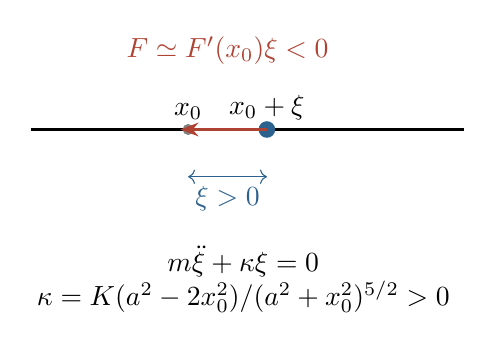
\begin{tikzpicture}
\draw[thick](-2,0)--(3.5,0);\fill[gray](0,0)circle(2pt);\node[above]at(0,0){$x_0$};
\fill[blue](1,0)circle(3pt);\node[above]at(1,0){$x_0+\xi$};
\draw[blue,<->](0,-.6)--node[below]{$\xi>0$}(1,-.6);
\draw[red,thick,-{Stealth}](1,0)--(-.1,0);\node[red]at(.5,1){$F\simeq F'(x_0)\xi<0$};
\node[align=center]at(.7,-1.9){$m\ddot\xi+\kappa\xi=0$\\$\kappa=K(a^2-2x_0^2)/(a^2+x_0^2)^{5/2}>0$};
\end{tikzpicture}
\end{document}
